\begin{titlepage}

%\centering


\begin{figure}
   \centering

\vfill
{\bfseries\Large
   Piccolo Manuale di LibreLogo\\
   Versione 4.1\\
   \vskip2cm
   Andreas R. Formiconi\\
   \vskip2cm
}    
\vfill

   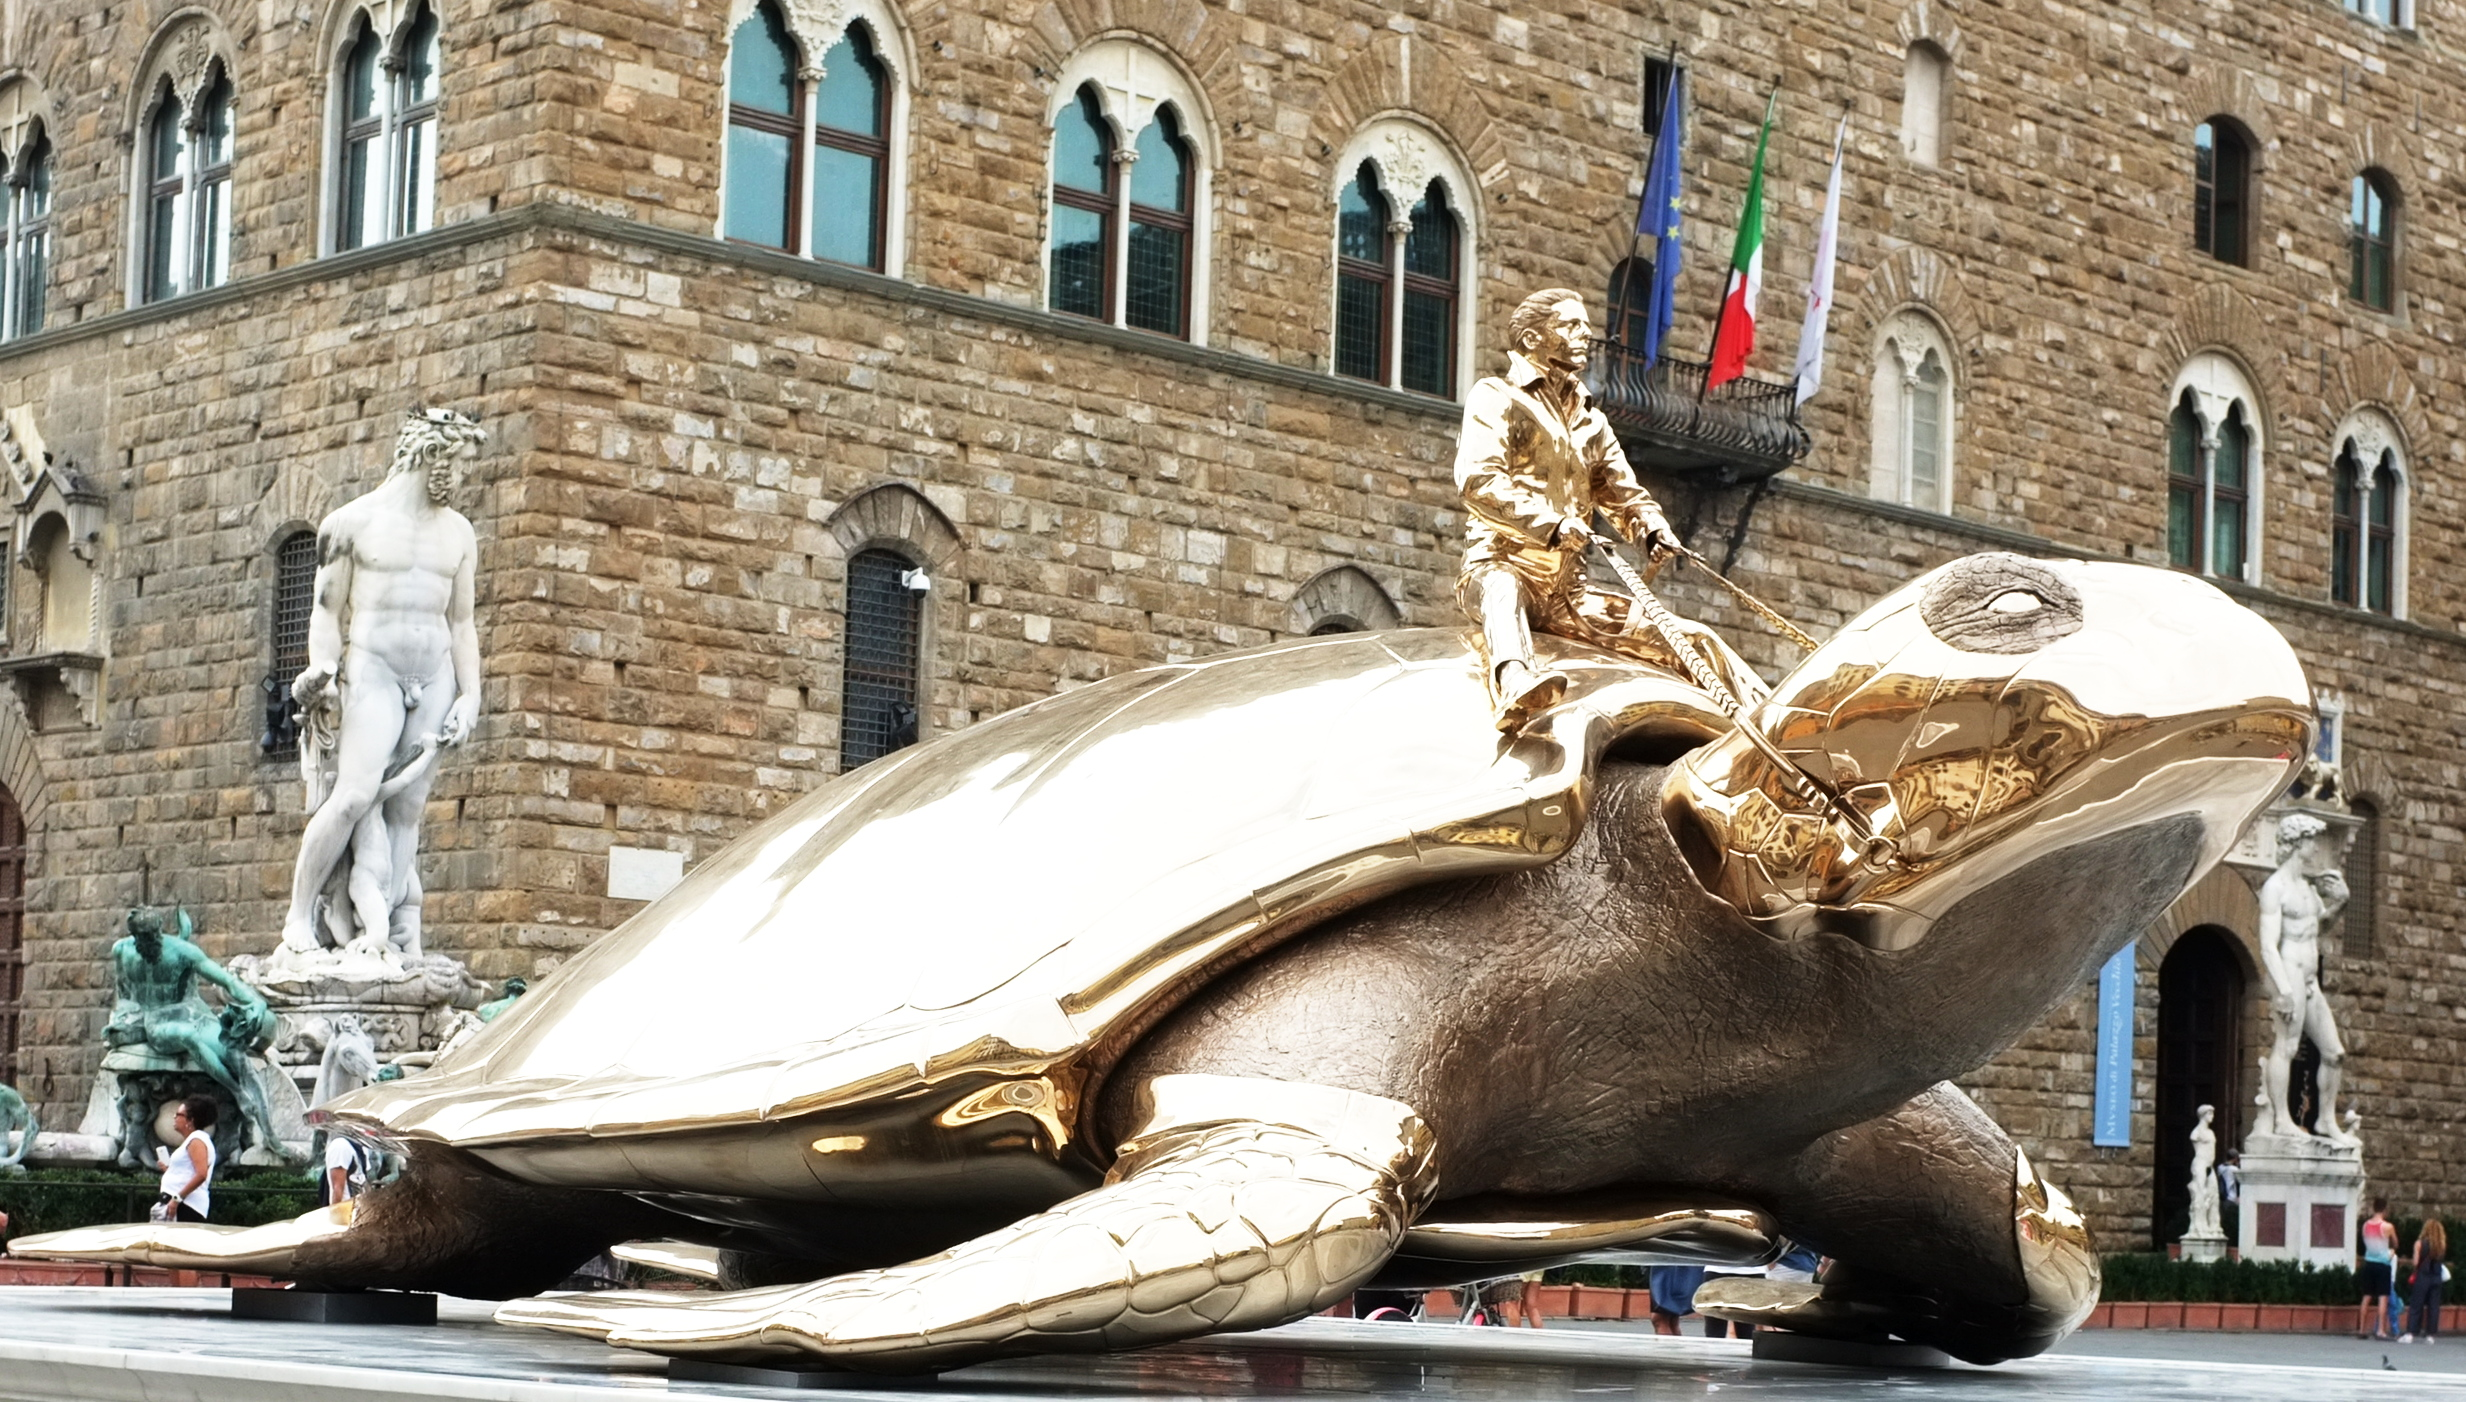
\includegraphics[width=3.0in]{utopia.jpg}
   \caption{Jan Fabre, "Searching for Utopia", 2003} 
   \label{utopia}


\vfill
{\bfseries \vskip4cm \small
Quest'opera è stata rilasciata con licenza Creative Commons Attribuzione 2.5 Italia. Per leggere una
copia della licenza visita il sito web http://creativecommons.org/licenses/by/2.5/it/ o spedisci una
lettera a Creative Commons, PO Box 1866, Mountain View, CA 94042, USA.\\
}    
\vfill

\end{figure}

\end{titlepage}


\section{Prefazione}
Questo piccolo manuale nasce per la necessità di fornire supporto di studio e consultazione nell'insegnamento “Laboratorio di Tecnologie Didattiche” al V anno del Corso di Laurea Magistrale a ciclo unico “Scienze della Formazione Primaria” e nell'insegnamento “Laboratorio di Gestione dei Processi Formativi” al II anno del Corso di Laurea Magistrale “Scienze dell'Educazione degli Adulti, della Formazione Continua e Scienze Pedagogiche”, presso l'Università di Firenze, e nell'insegnamento “Informatica” al I anno del Corso di Laurea Magistrale “Innovazione Educativa e Apprendimento Permanente” presso l'università telematica Italian University Line. Il manuale guida all'impiego del linguaggio Logo nella versione LibreLogo implementata all'interno del word processor Writer della suite di programmi di produttività personale LibreOffice. LibreLogo è un plugin disponibile di default in Writer a partire dalla versione 4.0 di LibreOffice. È stato scritto in linguaggio Python da László Németh. La documentazione disponibile si trova in http://librelogo.org, da dove, in particolare, si può scaricare una guida dei comandi di LibreLogo in italiano[1]. Per il resto, sfortunatamente e per quanto è a mia conoscenza sino ad oggi, la documentazione disponibile è tutta in ungherese, principalmente sotto forma di un manualetto conciso scritto dallo stesso László Németh[2] e da un manuale esteso scritto da Lakó Viktória[3]. È a quest'ultimo lavoro che, in una prima fase si è ispirato il presente piccolo manuale, senza tuttavia esserne una traduzione, per vari motivi. In primo luogo io non so l'ungherese e non posso quindi pretendere di poterne fare una vera traduzione e i tempi e le circostanze non mi consentono di avvalermi di un traduttore. Posso tuttavia seguirne le tracce, aiutandomi con i codici (anche se in ungherese quelli si possono imparare), le figure e Google Translate. Del resto, alla fine una traduzione pedissequa non sarebbe nemmeno desiderabile perché viene naturale riformulare il materiale in funzione degli obiettivi specifici e della propria visione della materia. Inoltre, nel corso della traduzione, mi è capitato sempre più spesso di seguire la traccia dei miei pensieri e, alla fine, è stato inevitabile tornare alla fonte primigenia, ovvero al testo con cui Seymour Papert descrisse per la prima volta compiutamente il pensiero che aveva dato origine a Logo, Mindstorms[4]. È così che ho introdotto la traduzione di due capitoli di Mindstorms: il secondo, “Mathofobia: the Fear of Learning”, e il terzo, “Turtle Geometry: A Mathematics Made for Learning”.

\begin{equation}
	    \label{simple_equation}
	        \alpha = \sqrt{ \beta }
\end{equation}

\subsection{sottosezione}
Bla bla


\section{Conclusione}
Eh...

